\documentclass[resume]{subfiles}


\begin{document}
\section{Firewall iptables}
Il est nécessaire d'activer netfilter dans la configuration du kernel. Un hook est une étape lors du passage d'une trame dans le stack de protocoles. Le framework netfilter sera appelé à chaque hook
\begin{figure}[H]
\centering
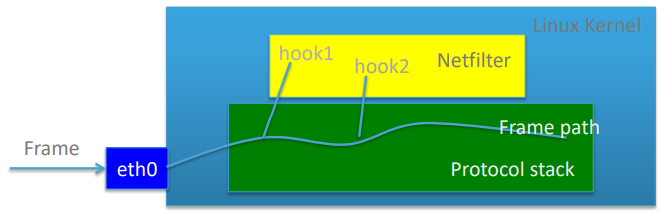
\includegraphics[width=0.8\columnwidth]{img_6.png}
\end{figure}
On peut configurer netfilter avec la commande \verb!iptables!. \verb!ebtables! permet de configurer la couche 2 uniquement (Linux bridge). \verb!nftables! vise à remplacer tout le framework
\begin{figure}[H]
\centering
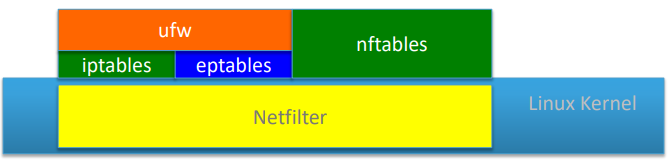
\includegraphics[width=0.6\columnwidth]{img_7.png}
\end{figure}
\subsection{Features}
\begin{enumerate}
\item Stateless packet filtering (table filter et ACCEPT, DROP, REJECT). Permet de protéger au niveau réseau (bloquage d'une ip en particulier, ou ports). Les paquets sont analysés de manière individuelle
\item Stateful packet filtering. Permet de protéger au niveau du paquet en fonction du contexte (précédents paquets). Il est possible d'accepter des paquets venant de l'extérieur seulement si ils sont des réponses à des requêtes venant de l'intérieur
\begin{itemize}
\item Utilisation de connection tables pour traiter les différentes parties des protocoles.
\item NEW : Nouveau paquet qui n'est pas lié à une connexion active
\item ESTABLISHED : Une connexion passe de NEW à ESTABLISHED losrque la connexion est validée par la direction opposée
\item RELATED : Paquets qui ne font pas partie d'une connexion existante mais qui sont liés à une autre. (Par exemple réponses ICMP pour une communication FTP).
\end{itemize}
\item Translation d'adresses / ports (NAT)
\item API pour autres applications
\end{enumerate}
\subsection{Chain}
la combinaison Chain-Table constitue les hooks
\paragraph{Chains} : INPUT, OUTPUT, FORWARD, PREROUTING, POSTROUTING
\subsubsection{Tables}
\begin{itemize}
\item raw
\item mangle (modification spéciales sur des paquets)
\item nat (consultée lorsqu'un paquet créé une nouvelle connexion)
\item filter (table de base)
\end{itemize}
\begin{figure}[H]
\centering
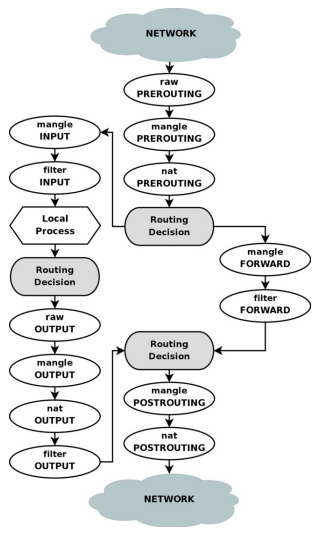
\includegraphics[width=3.50cm]{img_8.png}
\end{figure}
\subsection{NFQUEUE}
NFQUEUE permet de passer un paquet au userspace
\subsection{knockd}
Configuration dynamique du parefeu netfilter. Lorsque des séquences sont reconnues (par exemple des ports spécifiques), le pare-feu est ouvert.
\subsection{fwknop}
Même système que knockd mais il utilise le contenu des paquets TCP / UDP (frame SPA)

\subsection{Commande iptables}
\begin{center}
\verb!iptables -t table -COMMAND chain ... -j TARGET!
\end{center}

\end{document}